\documentclass[fontset=founder]{ucedubook}
\noprintanswers

\usepackage{tabularray}

\pagestyle{chapter}

\graphicspath{{figures}}

\ctexset{
  section = {
    number = \chinese{section},
    name = {,、}
  }
}



\begin{document}

\chapter*{2022年全国新高考I卷数学试题}

\section{单选题}

\begin{ti}
若集合$M = \Set{ x | \sqrt{x} < 4 }$,$N = \Set{ x | 3x \geq 1 }$,则$M \cap N =$(\qquad)

\begin{choices}
  \item $\Set{ x | 0 \leq x < 2 }$
  \item $\Set{ x | \frac{1}{3} \leq x < 2 }$
  \item $\Set{ x | 3 \leq x < 16 }$
  \item $\Set{ x | \frac{1}{3} \leq x < 16 }$
\end{choices}
\end{ti}


\begin{ti}
若$\mathrm{i}(1 - z) = 1$,则$z + \overline{z} =$(\qquad)

\begin{choices}
  \item $- 2$
  \item $- 1$
  \item $1$
  \item $2$
\end{choices}
\end{ti}


\begin{ti}
在$\triangle ABC$中,点$D$在边$AB$上,$BD = 2DA$.记$\overrightarrow{CA} = \overrightarrow{m}$,$\overrightarrow{CD} = \overrightarrow{n}$,则$\overrightarrow{CB} =$(\qquad)

\begin{choices}
  \item $3\overrightarrow{m} - 2\overrightarrow{n}$
  \item $- 2\overrightarrow{m} + 3\overrightarrow{n}$
  \item $3\overrightarrow{m} + 2\overrightarrow{n}$
  \item $2\overrightarrow{m} + 3\overrightarrow{n}$
\end{choices}
\end{ti}


\begin{ti}
南水北调工程缓解了北方一些地区水资源短缺问题,其中一部分水蓄入某水库.已知该水库水位为海拔$148.5\,\mathrm{m}$时,相应水面的面积为$140.0\,\mathrm{{km}^{2}}$;水位为海拔$157.5\,\mathrm{m}$时,相应水面的面积为$180.0\,\mathrm{{km}^{2}}$,将该水库在这两个水位间的形状看作一个棱台,则该水库水位从海拔$148.5\,\mathrm{m}$上升到$157.5\,\mathrm{m}$时,增加的水量约为($\sqrt{7} \approx 2.65$)(\qquad)

\begin{choices}
  \item $1.0 \times 10^{9}\,\mathrm{{m}^{3}}$
  \item $1.2 \times 10^{9}\,\mathrm{{m}^{3}}$
  \item $1.4 \times 10^{9}\,\mathrm{{m}^{3}}$
  \item $1.6 \times 10^{9}\,\mathrm{{m}^{3}}$
\end{choices}
\end{ti}


\begin{ti}
从$2$至$8$的$7$个整数中随机取$2$个不同的数,则这$2$个数互质的概率为(\qquad)

\begin{choices}
  \item $\frac{1}{6}$
  \item $\frac{1}{3}$
  \item $\frac{1}{2}$
  \item $\frac{2}{3}$
\end{choices}
\end{ti}


\begin{ti}
记函数$f(x) = \sin\left(\omega x + \frac{\pi}{4}\right) + b\;(\omega > 0)$的最小正周期为$T$.若$\frac{2\pi}{3} < T < \pi$,且$y = f(x)$的图象关于点$\left(\frac{3\pi}{2},2\right)$中心对称,则$f\left(\frac{\pi}{2}\right) =$(\qquad)

\begin{choices}
  \item $1$
  \item $\frac{3}{2}$
  \item $\frac{5}{2}$
  \item $3$
\end{choices}
\end{ti}


\begin{ti}
设$a = 0.1e^{0.1}$,$b = \frac{1}{9}$,$c = - \ln 0.9$,则(\qquad)

\begin{choices}
  \item $a < b < c$
  \item $c < b < a$
  \item $c < a < b$
  \item $a < c < b$
\end{choices}
\end{ti}


\begin{ti}
已知正四棱锥的侧棱长为$l$,其各顶点都在同一球面上.若该球的体积为$36\pi$,且$3 \leq l \leq 3\sqrt{3}$,则该正四棱锥体积的取值范围是(\qquad)

\begin{choices}
  \item $\left\lbrack 18,\frac{81}{4} \right\rbrack$
  \item $\left\lbrack \frac{27}{4},\frac{81}{4} \right\rbrack$
  \item $\left\lbrack \frac{27}{4},\frac{64}{3} \right\rbrack$
  \item $\lbrack 18,27\rbrack$
\end{choices}
\end{ti}


\newpageb
\section{多选题}

\begin{ti}
已知正方体$ABCD - A_{1}B_{1}C_{1}D_{1}$,则(\qquad)

\begin{choices}
  \item 直线$BC_{1}$与$DA_{1}$所成的角为$90{^\circ}$
  \item 直线$BC_{1}$与$CA_{1}$所成的角为$90{^\circ}$
  \item 直线$BC_{1}$与平面$BB_{1}D_{1}D$所成的角为$45{^\circ}$
  \item 直线$BC_{1}$与平面$ABCD$所成的角为$45{^\circ}$
\end{choices}
\end{ti}


\begin{ti}
已知函数$f(x) = x^{3} - x + 1$,则(\qquad)

\begin{choices}
  \item $f(x)$有两个极值点
  \item $f(x)$有三个零点
  \item 点$(0,1)$是曲线$y = f(x)$的对称中心
  \item 直线$y = 2x$是曲线$y = f(x)$的切线
\end{choices}
\end{ti}


\begin{ti}
已知$O$为坐标原点,点$A(1,1)$在抛物线$C:x^{2} = 2py\;(p > 0)$上,过点$B(0, - 1)$的直线交$C$于$P$,$Q$两点,则(\qquad)

\begin{choices}
  \item $C$的准线为$y = - 1$
  \item 直线$AB$与$C$相切
  \item $|OP| \cdot |OQ| > |OA|^{2}$
  \item $|BP| \cdot |BQ| > |BA|^{2}$
\end{choices}
\end{ti}


\begin{ti}
已知函数$f(x)$及其导函数$f'(x)$的定义域均为$R$,记$g(x) = f'(x)$,若$f\left( \frac{3}{2} - 2x \right)$,$g(2 + x)$均为偶函数,则(\qquad)

\begin{choices}
  \item $f(0) = 0$
  \item $g\left( - \frac{1}{2} \right) = 0$
  \item $f( - 1) = f(4)$
  \item $g( - 1) = g(2)$
\end{choices}
\end{ti}


\newpageb
\section{填空题}

\begin{ti}
$\left( 1 - \frac{y}{x} \right){(x + y)}^{8}$的展开式中$x^{2}y^{6}$的系数为\kong[8](用数字作答).
\end{ti}


\begin{ti}
写出与圆$x^{2} + y^{2} = 1$和${(x - 3)}^{2} + {(y - 4)}^{2} = 16$都相切的一条直线的方程\kong[8].
\end{ti}


\begin{ti}
若曲线$y = (x + a)\mathrm{e}^{x}$有两条过坐标原点的切线,则$a$的取值范围是\kong[8].
\end{ti}


\begin{ti}
已知椭圆$C:\frac{x^{2}}{a^{2}} + \frac{y^{2}}{b^{2}} = 1\;(a > b > 0)$,$C$的上顶点为$A$,两个焦点为$F_{1}$,$F_{2}$,离心率为$\frac{1}{2}$.过$F_{1}$且垂直于$AF_{2}$的直线与$C$交于$D$,$E$两点,$|DE| = 6$,则$\triangle ADE$的周长是\kong[8].
\end{ti}


\newpageb
\section{解答题}

\begin{ti}[.5]
记$S_{n}$为数列$\left\{ a_{n} \right\}$的前$n$项和,已知$a_{1} = 1$,$\left\{ \frac{S_{n}}{a_{n}} \right\}$是公差为$\frac{1}{3}$的等差数列.

(1)求$\left\{ a_{n} \right\}$的通项公式;

(2)证明:$\frac{1}{a_{1}} + \frac{1}{a_{2}} + \cdots + \frac{1}{a_{n}} < 2$.
\end{ti}


\begin{ti}[.5]
记$\triangle ABC$的内角$A$,$B$,$C$的对边分别为$a$,$b$,$c$,已知$\frac{\cos A}{1 + \sin A} = \frac{\sin 2B}{1 + \cos 2B}$.

(1)若$C = \frac{2\pi}{3}$,求$B$;

(2)求$\frac{a^{2} + b^{2}}{c^{2}}$的最小值.
\end{ti}


\begin{ti}[.5]
如图,直三棱柱$ABC - A_{1}B_{1}C_{1}$的体积为4,$\triangle A_{1}BC$的面积为$2\sqrt{2}$.

(1)求$A$到平面$A_{1}BC$的距离;

(2)设$D$为$A_{1}C$的中点,$AA_{1} = AB$,平面$A_{1}BC\perp$平面$ABB_{1}A_{1}$,求二面角$A - BD - C$的正弦值.

\hfill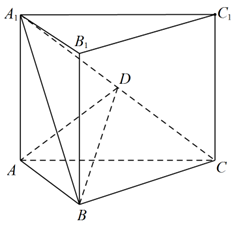
\includegraphics[]{新高考I-19.png}
\end{ti}

\newpageb


\begin{ti}[.5]
一医疗团队为研究某地的一种地方性疾病与当地居民的卫生习惯(卫生习惯分为良好和不够良好两类)的关系,在已患该疾病的病例中随机调查了100例(称为病例组),同时在未患该疾病的人群中随机调查了$100$人(称为对照组),得到如下数据:

\begin{center}
  \begin{tblr}{|c|c|c|}
    \hline
    & 不够良好 & 良好 \\
    \hline
    病例组 & 40 & 60 \\
    \hline
    对照组 & 10 & 90 \\
    \hline
  \end{tblr}
\end{center}

(1)能否有$99\%$的把握认为患该疾病群体与未患该疾病群体的卫生习惯有差异?

(2)从该地的人群中任选一人,$A$表示事件``选到的人卫生习惯不够良好'',$B$表示事件``选到的人患有该疾病''.$\frac{P(B|A)}{P(\overline{B}|A)}$与$\frac{P(B|\overline{A})}{P(\overline{B}|\overline{A})}$的比值是卫生习惯不够良好对患该疾病风险程度的一项度量指标,记该指标为$R$.

(ⅰ)证明:$R = \frac{P(A|B)}{P(\overline{A}|B)} \cdot \frac{P(\overline{A}|\overline{B})}{P(A|\overline{B})}$;

(ⅱ)利用该调查数据,给出$P(A|B),P(A|\overline{B})$的估计值,并利用(ⅰ)的结果给出$R$的估计值.

附$K^{2} = \frac{n{(ad - bc)}^{2}}{(a + b)(c + d)(a + c)(b + d)}$,


\begin{tblr}{|c|c|c|c|}
  \hline
  $P\left( K^{2} \geq k \right)$ & 0.050 & 0.010 & 0.001 \\
  \hline
  $k$ & 3.841 & 6.635 & 10.828 \\
  \hline
\end{tblr}
\end{ti}

\newpageb


\begin{ti}[.5]
已知点$A(2,1)$在双曲线$C:\frac{x^{2}}{a^{2}} - \frac{y^{2}}{a^{2} - 1} = 1(a > 1)$上,直线$l$交$C$于$P$,$Q$两点,直线$AP,AQ$的斜率之和为$0$.

(1)求$l$的斜率;

(2)若$\tan\angle PAQ = 2\sqrt{2}$,求$\triangle PAQ$的面积.
\end{ti}

\newpageb


\begin{ti}[.5]
已知函数$f(x) = e^{x} - ax$和$g(x) = ax - \ln x$有相同的最小值.

(1)求$a$;

(2)证明:存在直线$y = b$,其与两条曲线$y = f(x)$和$y = g(x)$共有三个不同的交点,并且从左到右的三个交点的横坐标成等差数列.
\end{ti}



\end{document}